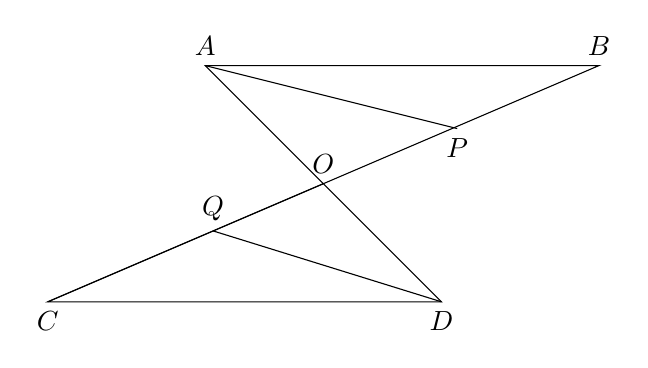
\begin{tikzpicture} 
        \coordinate (A) at (0, 3) {};
        \coordinate (B) at (5, 3) {};
        \coordinate (C) at (-2, 0) {};
        \coordinate (D) at (3, 0) {};
        \coordinate (P) at (3.2, 2.2) {};
        \coordinate (Q) at (0.1, 0.9) {};
        \coordinate (O) at (1.5, 1.5) {};
        \draw (A)node[above]{$A$}--(B)node[above]{$B$}--(C)node[below]{$C$}--(D)node[below]{$D$}--cycle;
        \draw (C)node[below]{}--(O)node[above]{$O$};
        \draw (A)node[above]{}--(P)node[below]{$P$};
        \draw (D)node[below]{}--(Q)node[above]{$Q$};
\end{tikzpicture}